% $Id: circuit.tex 9373 2021-08-30 21:03:39Z mskala $

%
% MSK 012 circuit explanation
% Copyright (C) 2018  Matthew Skala
%
% This program is free software: you can redistribute it and/or modify
% it under the terms of the GNU General Public License as published by
% the Free Software Foundation, version 3.
%
% This program is distributed in the hope that it will be useful,
% but WITHOUT ANY WARRANTY; without even the implied warranty of
% MERCHANTABILITY or FITNESS FOR A PARTICULAR PURPOSE.  See the
% GNU General Public License for more details.
%
% You should have received a copy of the GNU General Public License
% along with this program.  If not, see <http://www.gnu.org/licenses/>.
%
% Matthew Skala
% https://northcoastsynthesis.com/
% mskala@northcoastsynthesis.com
%

\chapter{Circuit explanation}

The design concept for the MSK~012 was to explore generating a classic ADSR
envelope with logic as simple as possible, and in particular, a minimum
number of transistors.  Many ADSR envelope generators would use op amps for
computing the necessary time-varying voltages, or even just throw in a
microcontroller and do everything in software, and either of those
expedients might keep the \emph{parts} count down by using parts containing
dozens or thousands of transistors; but how far can we get with a very small
\emph{transistor} count?

\section{Inverters and multivibrators}

One simple circuit is used repeatedly in this module in varying forms.  It
looks something like this.

{\centering\input{rtlinv.tex}\par}

This circuit is the simplest possible logic gate in a system of
\emph{resistor-transistor logic} (RTL) where logic ``1'' is represented by
the power supply voltage through a few tens of kiloohms of resistance, and
logic ``0'' is represented by a low impedance with a low voltage drop to
ground.

Suppose we apply logic ``1'' to the input.  Current flows into the base of
the transistor (a few hundred microamps), the transistor switches on, in
saturation mode because its base current multiplied by its gain works out to
far more than the current available through the resistor, and so the output
(which is just the collector of the transistor) goes to the saturation
voltage of the transistor, which will be something like 0.3V.  The
transistor is capable of absorbing a signficant amount of additional current
through its collector without much increasing its voltage drop, so the
output of the circuit has a low impedance.  The output is thus a perfect RTL
``0.''

Now suppose instead we apply a logic ``0'' to the input.  The base of the
transistor is held at about 0.3V, which is below its turn-on voltage (typically about
0.7V), so the transistor does not pass any significant current, and the
power supply voltage is exposed to the circuit output through the
39k$\Omega$ resistor, therefore constituting an RTL ``1.''  In either case,
the circuit fed with one logic state at the input generates the other at the
output; it is an RTL \emph{inverter}.

Now consider two inverters connected in a loop.

{\centering\input{bistable.tex}\par}

If the input to the first inverter is logic ``0,'' its output will be logic
``1,'' which causes the output of the second inverter to be logic ``0,''
feeding back into and reinforcing the existing state of the first inverter's
input.  That is a stable state for the system.  If the input to the first
inverter were ``1,'' that is a second distinct stable state:  first
inverter's output goes to ``0,'' second inverter's output goes to ``1,'' and
that reinforces the original ``1.''  Once it is in one of these states the
circuit will reliably remain there; if it is temporarily somewhere else (for
instance, during startup) it will quickly fall into one of the two stable
states and then stay fixed.  A circuit of this type is called a
\emph{bistable multivibrator}; bistable because it has two stable states,
multivibrator from an archaic naming convention for switching
circuits coined in the early 20th Century.

In order to make this circuit really useful, we need to modify it in some
way (usually by adding some more resistors) to allow an external input to
temporarily overcome the feedback loop and force the circuit into a chosen
state.  Then when the external input is no longer strong enough to force it
into one state, the multivibrator will hold its previously-set state until
something else changes to switch it to the other state.  Its basic
usefulness, then, is as a one-bit memory that retains a logic state.  The
MSK~012 uses three such one-bit memories to keep track of the envelope
cycle.

\section{Input Schmitt trigger}

The gate control voltage coming into the module first goes through the input
Schmitt trigger, shown in Figure~\ref{fig:input-schmitt}.  This section
conditions it into a well-behaved logic level; although the gate voltage
might be slowly varying and anywhere between the power voltages ($\pm$12V),
we need a straightforward logic ``1'' or ``0'' with sharp transitions to
drive the rest of the module.

\begin{figure*}
  \centering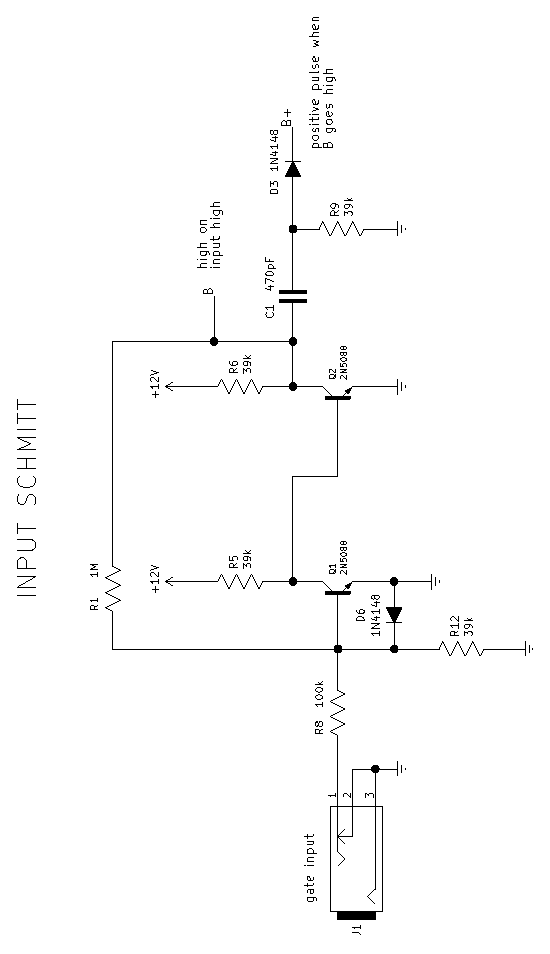
\includegraphics[angle=-90]{input-schmitt}\par
  \caption{Input Schmitt trigger}
  \label{fig:input-schmitt}
\end{figure*}

The input Schmitt trigger is a basic multivibrator as described in the
previous section, made up of two RTL inverters, with a resistor network
driving the input of the first one.  For sufficiently high input voltages
(that is, over about 2V) the input forces the multivibrator into the logic
``1'' state.  For sufficiently low input voltages (below about 1V), the
multivibrator is forced into the ``0'' state.  In between those thresholds,
the voltage divider formed by R8 and R12 would have an output voltage
sufficiently near Q1's switching voltage that the feedback through R1 is
sufficient to keep the multivibrator in its current state, whichever that
is.  The name \emph{Schmitt trigger} refers to this general kind of
switching circuit where there are two input thresholds and after switching,
the input must move some amount to hit the other one before it can switch
again.

The current state of the input Schmitt trigger appears as the RTL signal
labelled B on the schematic, but there is also an edge detector formed
by C1, R9, and D3.  When the gate input goes above 2V, causing B to become
high, current flows through C1 and D3 to create a pulse of current into the
signal labelled B$+$.  That happens only on the low-to-high transition, for
a few microseconds.  The current charges the capacitor, so the pulse dies
away, and then when B switches in the opposite direction, the diode blocks
the current so there is no negative pulse, and the capacitor discharges
through R9.  The pulse output B$+$ is used elsewhere in the module to switch
the attack flip-flop.

Note D6, from ground to the base of Q1.  This diode is meant to protect the
transistor from breakdown of its base-emitter junction in the case of a
large negative voltage at the module input.  At the rated worst case input
of $-$12V, the network of R1, R8, and R12 could bring the transistor base to
about $-$3.3V, which exceeds the 2N5088's rated limit of $-$3.0V.  The diode
limits the base voltage to no lower than $-$0.6V.

\section{Output Schmitt trigger}

There is another Schmitt trigger connected to the module output and shown in
Figure~\ref{fig:output-schmitt}.

\begin{figure*}
  \centering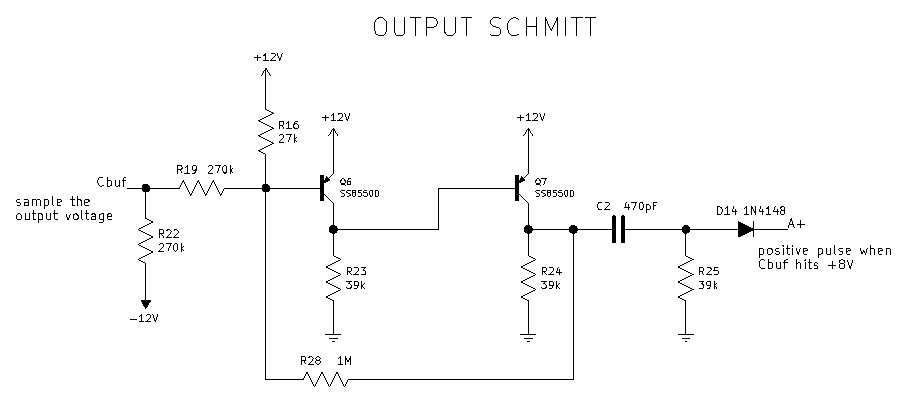
\includegraphics{output-schmitt}\par
  \caption{Output Schmitt trigger}
  \label{fig:output-schmitt}
\end{figure*}

This one is used to detect the end of the attack phase, and it is built with
PNP transistors (essentially, all the polarities reversed from those of the
input Schmitt trigger) in order to better handle switching at a voltage near
the positive supply.  The resistor network at the input of this section is
similar to that of the input Schmitt trigger, with the addition of R22,
which drains some current into the negative supply to prevent the
current through R16 and R19 from artificially raising the module's output
voltage.

When the module's output reaches about 8V, marking the end of the attack,
this Schmitt trigger switches into the ``1'' state.  The plain state of the
output Schmitt trigger is not used elsewhere in the module, but there is
another edge detector (C2, R25, D14) which generates a pulse into the signal
marked A$+$ when the end-of-attack event happens.  The Schmitt trigger will
turn off again (ready to detect another attack) after the output voltage
drops a couple of volts.

\section{Attack flip-flop}

Both input and output Schmitt triggers feed into the attack flip-flip, which
keeps track of whether the module is currently in the attack phase, as shown
in Figure~\ref{fig:attack-ff}.

\begin{figure}
  \centering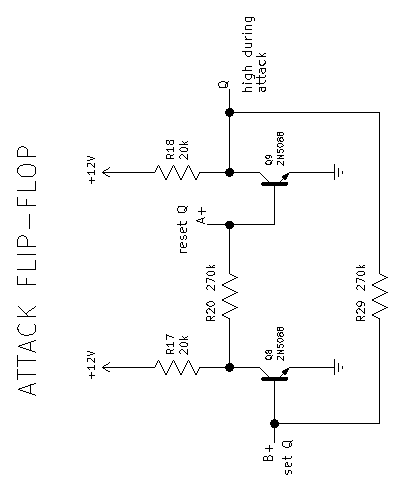
\includegraphics[angle=-90]{attack-ff}\par
  \caption{Attack flip-flop}
  \label{fig:attack-ff}
\end{figure}

This is a basic bistable multivibrator with 270k$\Omega$ resistors between
the stages, weakening the signals so that although they remain strong
enough to hold the state without external input, they can be overridden by
pulses from the Schmitt triggers.  At the start of the external gate signal,
there is a pulse on B$+$ from the input Schmitt trigger, setting the flip-flop
into the ``1'' state (start of attack).  When the output voltage reaches about 8V, there is a
pulse on A$+$ from the output Schmitt trigger, resetting the flip-flop to
the ``0'' state.  The current state is available as the signal marked Q.

Note that the collector resistors (R17 and R18) in this flip-flop are a
little smaller than elsewhere in the module, at 20k$\Omega$ instead of
39k$\Omega$.  The value of R18 is reduced in order to be sure it can provide
enough current to the ADSR driver, which consumes this signal; and the value
of R17 is made to match it so that the overall static current consumption of
this section will not change with the state of the flip-flop, reducing the
possibility for audio-rate spikes to be generated in the power system.

\section{ADSR driver}

The section called the ADSR driver (Figure~\ref{fig:adsr-driver}) does most
of the work of shaping the envelope.

\begin{figure*}
  \centering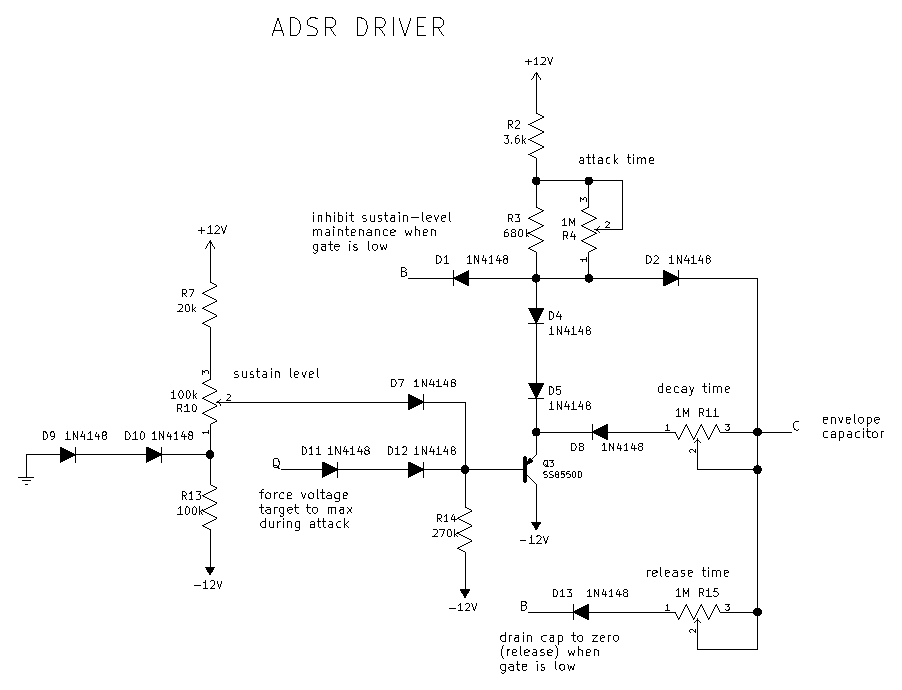
\includegraphics{adsr-driver}\par
  \caption{ADSR driver}
  \label{fig:adsr-driver}
\end{figure*}

First, note the connection labelled C, which goes to the capacitor in the
output buffer section.  This section's output is in the form of a
bidirectional current that charges or discharges the capacitor at different
rates.  Its input is two logic signals:  Q from the attack flip-flop, which
is high from the start of the gate until the module output reaches about 8V,
and B from the input Schmitt trigger, which is high throughout the time the
input gate is high.

The ADSR driver's operation is best understood by looking at one state at a
time.  First, suppose the input gate is low and has been for a long time. 
Both B and Q are low, and the envelope capacitor is at or near 0V.  With B
low, current from R2, R3, and R4 flows through D1 into B, and the anode of
D1 remains low enough that D2, D4, and D5 are reverse-biased or at least not
sufficiently forward-biased to overcome their forward voltages and start
conducting.  Current flows from $+$12V to $-$12V through R7, some part of
R10, D7, and R14, and doing the math, this puts the base of Q3 a little
above ground, which means its emitter will be as well, and then D4, D5, and
D8 are reverse-biased, blocking D11 out of the circuit.  The only remaining
path for current to or from the output is through R15 and D13 to the
near-ground B signal; that keeps the envelope capacitor near ground. 
Technically, its minimum voltage will be about $+$1.0V, that being one diode
drop for D13 and one saturated transistor voltage for Q2 in the input Schmitt
trigger, but this is compensated by an offset in the output buffer to bring
the actual output of the module near zero.

Now, suppose the input gate goes high.  The B signal goes high, which
triggers a pulse on the B$+$ signal, setting the attack flip-flop, and so Q
goes high as well.  With B high, D13 is reverse-biased, taking R15 out of
the circuit.  With Q high, the base of Q3 is kept high, which keeps D4, D5,
and D8 reverse-biased and takes R11 out of the circuit.  Then the envelope
capacitor is exposed to current from the resistor
network of R2, R3, and R4 through D2.  The capacitor starts to charge at a
rate controlled by the setting of R4; this is the attack phase of the
envelope.

When the envelope capacitor has charged enough for the output of the module
to exceed about 8V, the output Schmitt trigger fires, generating a pulse on
A$+$ which switches the attack flip-flop and causes Q to go low.  Then the
components connected to the base of Q3 come into play.

The potentiometer R10 is adjusted to the sustain voltage, with a proper
offset for diode and transistor drops elsewhere in the circuit.  Its low end
is kept at about $-$1.2V by forward-biased D9 and D10, serving as primitive
voltage regulators with current through R13 keeping them forward-biased. 
The high end of R10 is separated from the positive supply by R7, keeping the
maximum sustain level at about the 8V maximum of the attack phase.  (From
breadboard experiments: setting a sustain voltage higher than the top of the
attack doesn't break anything, but results in strange and probably
undesirable envelope shapes.) The sustain voltage goes through D7 (which
serves to block it from loading the Q signal when Q is high) to the base of
Q3.  With Q blocked by reverse-biased D11 and D12, Q3 functions as an
emitter follower, holding its emitter at the sustain level.

Current flows from the envelope capacitor through R11 and D8 into Q3.  The
envelope capacitor discharges in a nice exponential-decay curve at a rate
set by R11 until it hits the sustain voltage.  Current from the attack-rate
network is bypassed through D4 and D5 to also drain into Q3; note that D4
and D5 maintain a voltage of two diode drops, whereas the voltage needed
across D2, R11, and D8 to turn on the diodes will inevitably be more than
that due to the voltage drop across R11 during decay, so current from the
attack network does not go into the capacitor to gum things up there; only
the decay potentiometer is in play during the decay phase.

However, suppose after the decay phase the
gate remains high for a long time.  There may be a small amount of leakage
from the envelope capacitor, causing its voltage to droop.  \emph{Then}, as
the voltage on the envelope capacitor drops below the intended sustain
level, D2 will start to conduct, stealing current from D4 and D5.  Note that
the anode of D4 is kept two diode drops above the emitter of Q3, so this
effect will kick in to prevent the capacitor going below one diode drop from
the emitter of Q3; that is, exactly the sustain level.  Current through R11
drops the voltage to the sustain level during the decay, but current from
the attack circuit prevents it from dropping any further in case of a long
sustain, and the current available corresponding to the attack speed is
always enough to compensate for current lost from the capacitor elsewhere in
the module.

When the gate input eventually goes low again, we are back where we started. 
The B signal goes low, stealing current from the attack network and
preventing it from holding the capacitor up at the sustain level.  The decay
circuit is blocked off by the emitter of Q3 being at the sustain level,
thus unable to increase the capacitor voltage or decrease it any further
than that level.  The only remaining path for current to or from the
envelope capacitor is through D13 and R15, draining it at the release rate
until it reaches its minimum level.

\section{Output buffer}

The output buffer, shown in Figure~\ref{fig:output-buffer}, integrates the
current output of the ADSR driver into a voltage and buffers it, both for
the output Schmitt trigger and the output of the whole module.

\begin{figure}
  \centering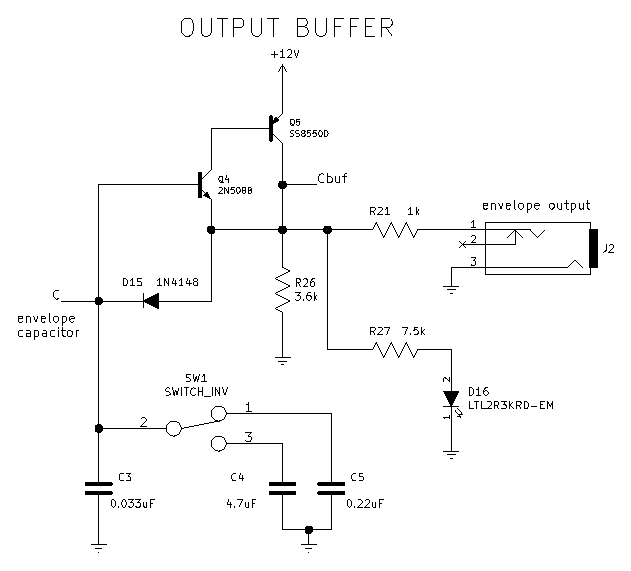
\includegraphics[scale=0.8]{output-buffer}\par
  \caption{Output buffer}
  \label{fig:output-buffer}
\end{figure}

The ``envelope capacitor'' may really be two; it consists of the 0.033$\mu$F
capacitor C3, possibly in parallel with C4 or C5.  The three-position switch
allows choosing to use one of those, or neither of them, for total
nominal capacitance of 0.033$\mu$F, 0.253$\mu$F, or 4.733$\mu$F (though
tolerances mean that the larger numbers are not precise to the stated number
of digits).

Transistors Q4 and Q5 (one PNP, one NPN) form a \emph{Sziklai pair}, which
functions much like a single NPN transistor of very high gain (equal to the
gain of its two transistors multiplied together).  The extra gain is needed
because even with the high-gain transistors I specify, a single transistor
would draw too much current from the envelope capacitor and disrupt the
envelope shape at low speeds, when biased to produce the desired amount of
output current.  The diode D15 protects Q4 from reverse bias, much like the
similar diode at the module input, in the case of someone shorting the
module output into the positive power supply or similar while the output is
being driven low.  The Sziklai pair combined with R26 is an emitter follower
that simply generates the desired output voltage, removing the offset from
the capacitor voltage.

From the emitter of the Sziklai pair, the output voltage goes to the output
Schmitt trigger to detect the end of the attack phase; through a
current-limiting resistor R21 to the output jack of the module; and through
another current-limiting resistor R27 to supply the LED D16.  Note the high
value of R27, which is not an error; the specified LED is a high-efficiency
type being operated significantly below its maximum rated current so as
not to be annoyingly bright.  The target is about 825$\mu$A when the
envelope hits 8V.